\chapter{基于有监督字典学习的OCT图像病态定位算法}

\section{方法概述} % (fold)
\label{sec:methodOverview}

    考虑一个简单场景:有一个非线性函数族,函数组中的函数形式未知,可能有多种函数类别,如何从中提取其中的线性成分。一个直观方法是使用最小二乘法拟合非线性函数族,找到与该非线性函数误差最小的线性函数。本方法的思想即基于以上基础的观察思路。观察到,无论病变位置种类如何不同,健康图像的形态总是在一定子空间内的。因此,当拥有一组病态图像,且不知道病变种类的条件下,本方法企图拟合一个未病变的健康图像,使重建的健康图像尽量与原图像相近。用病态图像减去重建健康图像,即推测得到病态位置。

    但是,仅仅在像素空间中使用欧氏距离拟合,由于维数太高以及各维之间有很高的相关性,简单的最小二乘法不能应用于本任务的场景。因此需要提取图像特征,使得特征满足:1. 不同特征之间减少相关性。2. 提取的特征有判别性。 3. 根据特征可以恢复到原像素空间中。 

    本文的总体算法流程如图~\ref{fig:pipeline}:
    \begin{figure} % use float package if you want it here
      \centering
      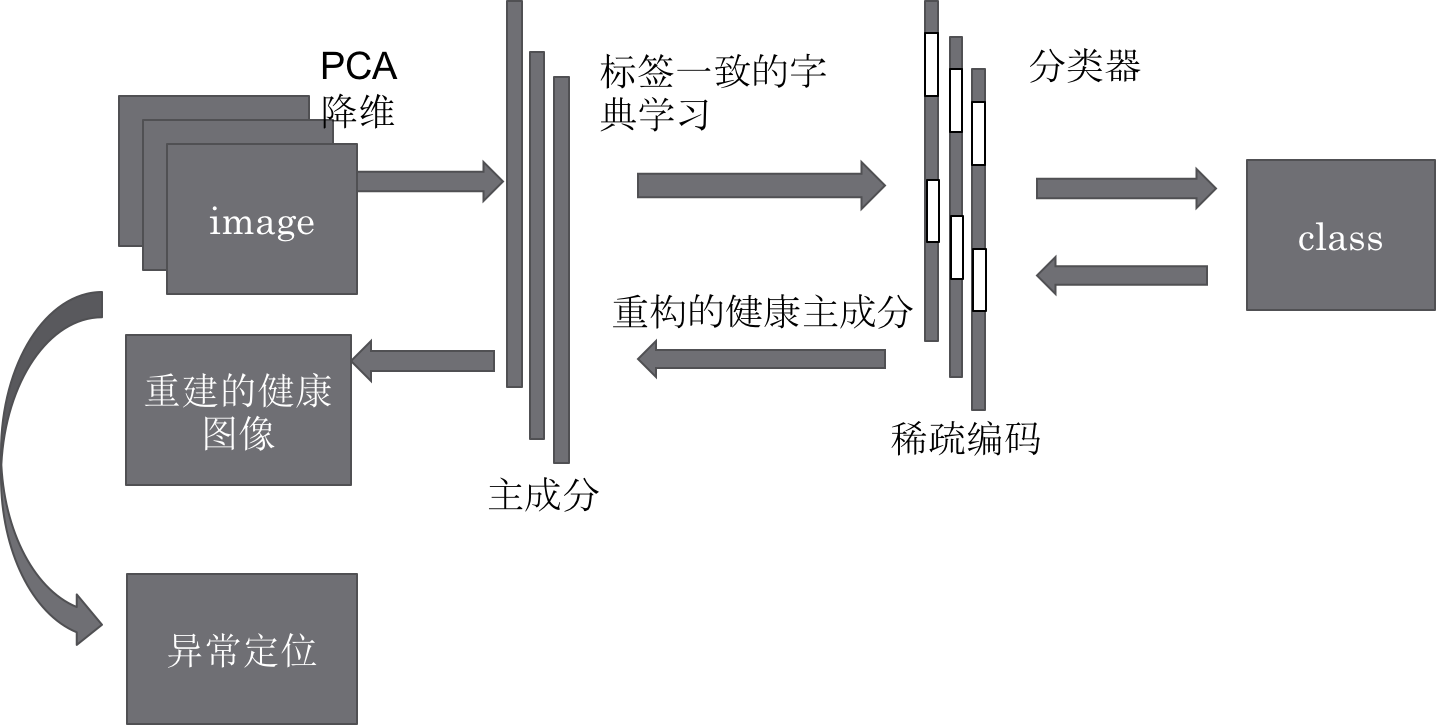
\includegraphics[width=\textwidth]{pipeline}
      \caption{算法流程图}
      \label{fig:pipeline}
    \end{figure}
    首先通过主成分分析对图片进行降维,这一步除了降低维数,还减少了各维之间的相关性。接着,对降维后的主成分表示学习一个标签一致的字典,和每个样本的稀疏表示,使特征具有稀疏性和较强判别性。对于如此特征,用一个线性分类器就可以得到较好的分类表现。在该特征空间中,找到健康图像构成的子空间,在其中欧氏距离意义下,拟合病态图片的特征,即找到对应的健康因素。然后再重构回健康的主成分,并重构像素空间中,推测的健康图像。 最后,用原图像减去健康图像,得到病态定位。

    本章将从数据降噪、对齐等预处理开始(~\ref{sec:Preprocessing}节),重点阐述主成分降维的方法和大数据集实现(~\ref{sec:pcaDR}节),标签一致字典学习和稀疏编码的原理和算法(~\ref{sec:lc-ksvd}节),以及逆向健康重建过程(~\ref{sec:norm-recon}节)。读者应重点关注采用该方法的动机,以及为本应用场景所做的特别改进。


% section _ (end)

% put to implementation detail
\section{数据预处理}
\label{sec:Preprocessing}

    对于中等规模的数据集的方法,对于空间对齐的要求较高。数据预处理主要是解决这个问题,同时,它还对图片做降噪、裁剪、齐次化这些基本操作。理想状态下,预处理后的图像视网膜中心凹处于中心位置,RPE层被拉直。目前有方法\cite{srinivasan2014fully}先寻找RPE层,然后平展该层,但是该方法不能处理RPE层严重变形的情况\cite{sun2017fully}.还有方法\cite{liu2011automated}用二次函数对OCT图像拟合,但是却难以处理严重水肿的情况。文献\inlinecite{sun2017fully} 提出了适用范围较广的预处理算法。本算法采用其预处理方法。

    先使用BM3D方法对原图降噪\cite{dabov2007image},然后,通过灰度阈值找到视网膜层,并做二值化,保留高于阈值,舍弃低于阈值的部位。接着通过做形态学的闭合运算,找到视网膜层的轮廓。对该视网膜层的轮廓蒙版做函数拟合,具体采用的拟合函数算法如图~\ref{fig:preprocess}.最后,将图像根据拟合函数拉直平展,裁剪,放缩到$512\times 128$的单通道黑白图像。
    \begin{figure}[htb] % use float package if you want it here
      \centering
      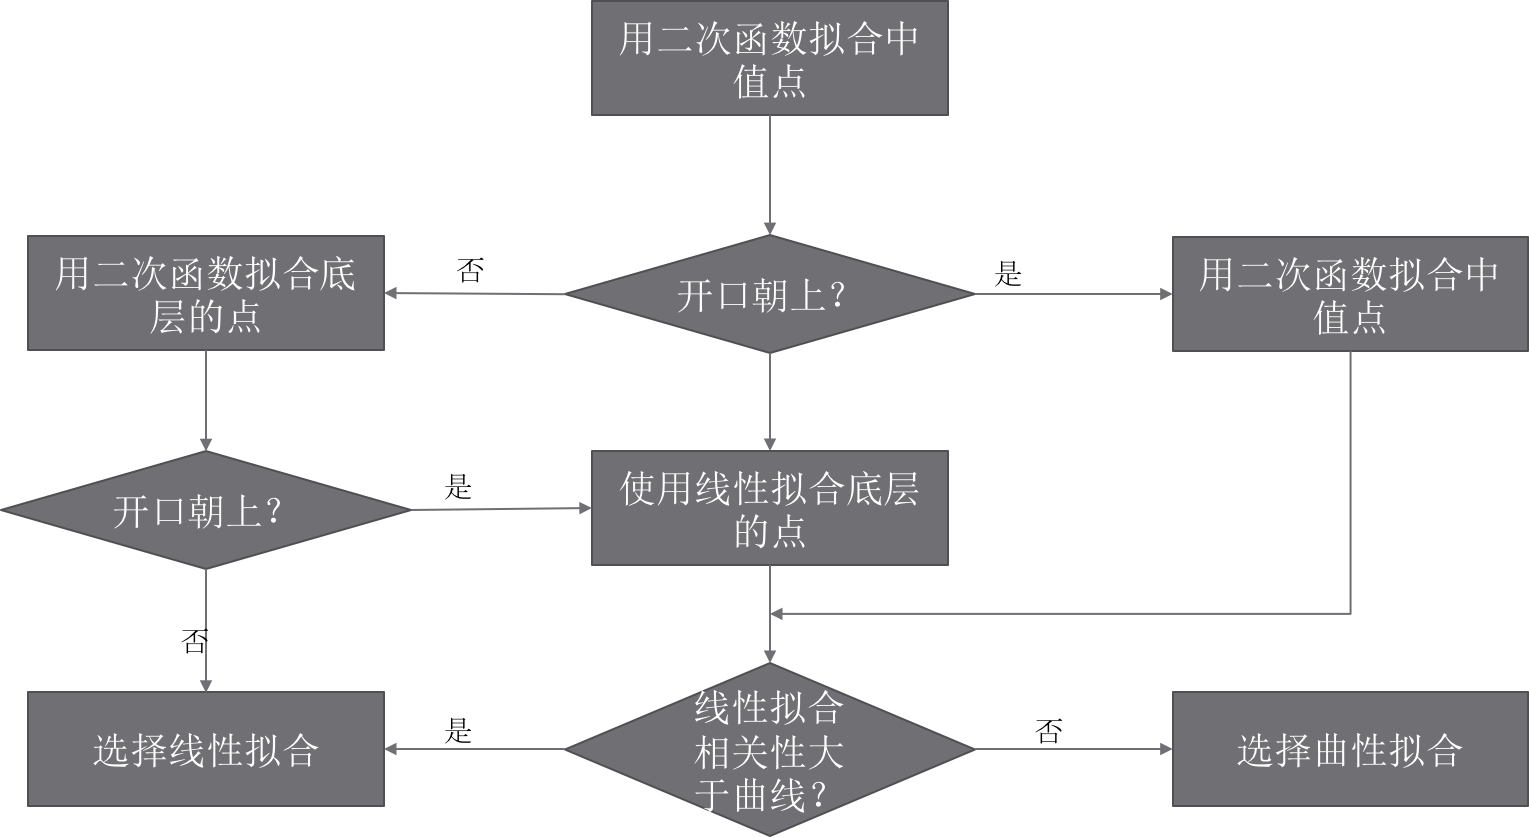
\includegraphics[width=\textwidth]{preprocess}
      \caption{数据预处理拟合算法}
      \label{fig:preprocess}
    \end{figure}

    \begin{figure}[htb]
      \centering%
      \subcaptionbox{\label{fig:origin}} %标题的长度,超过则会换行,如下一个小图。
        {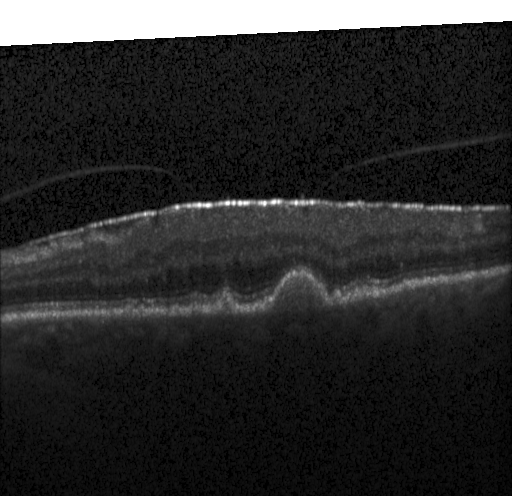
\includegraphics[width=.25 \textwidth]{origin}} %
      \subcaptionbox{\label{fig:aligned}} %标题的长度,超过则会换行,如下一个小图。
        {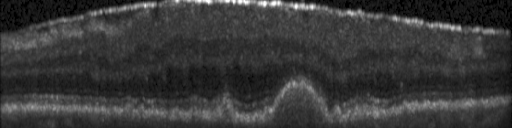
\includegraphics[width=.7\textwidth]{aligned}} \\
      \caption[数据预处理]{数据预处理。原始数据如图(a),经过降噪,过滤,拟合,拉伸,放缩等运算后得到$512\times 128$的图像如(b),后者将组成训练集} 
      \label{fig:origin-pre}
    \end{figure}


\section{基于PCA降维提取的特征图像}
\label{sec:pcaDR}
    \subsection{动机}
    把图像向量化是表达图像的基本手段。最直观的方法是在像素空间,直接把一个$N \times M$的图像,拉伸成$N\cdot M$维的 向量。但是,这种直观的方法,在高维空间中却会出现以下两个主要问题:
    \begin{enumerate}
        \item 计算量过大
        \item 在高维空间中,常用的距离,如欧式距离等,会降低识别性。
    \end{enumerate}
    有许多工作表明%\cite{dr-pca}
    降维是提高图像特征表达性能,也有一定的生物学基础\cite{olshausen1997sparse},它是提高识别率的有效方法。
    

    \subsection{PCA方法概述}
    主成分分析,(Principal Components Analysis,PCA)是一种非常直观但有效的降维手段。它寻找的是一个正交线性投影$R$,原来的空间通过$R$投影到低维空间上,使得数据在低维空间上的坐标轴方向上方差最大,且方差大小按照低维空间中坐标轴的顺序依次递减。它的数学表达如下,若$X \in \mathbb{R}^{N \times p}  $是一组观察数据,每一行代表一次观察,每次观察有p个变量。且$X$中每个变量的算术均值等于0。$R \in \mathbb{R} ^{p \times m}, (m \leqslant p) $ 是投影变换,将p维空间投影到m维空间中,投影后得到$\hat{X} = X\cdot R \in \mathbb{R}^{N \times m}$ 。$R = (r_1, r_2, \dots, r_m)$ 中 $r_i$ 满足 $ \|r_i\| = 1$ 且 $r_i \cdot r_j = 0$。从另一个几何空间的角度,也可以把$r_i$理解为投影后空间第i维坐标轴在原空间中的方向。根据定义,R的第1维坐标轴方向$r_{1}$满足
    \begin{equation}
    \label{eq:pcar1}
    \begin{split}
        r_{1} & = \mathop{\arg\max}_{\|r\|=1} (\sum_i(\hat{x} _i)^2 \\
        & = \mathop{\arg\max}_{\|r\| = 1}(\sum_i(x_{i}\cdot r)^2) \\
        & = \mathop{\arg\max} _{\|r\|=1} \|Xr\|^2 \\
        & = \mathop{arg\max}_{\|r\|= 1} (r^TX^TXw) \\
        & = \mathop{\arg\max} (\frac{r^TX^TXr}{r^Tr}) 
    \end{split}
    \end{equation}
    这是雷诺公式\cite{trefethen1997numerical}的形式,由线性代数的知识我们知道,$r_1$就是对称矩阵$X^TX$的最大特征值所对应的特征向量的方向。对于$r_i, i > 1$的情况,在求出第$k-1$维坐标轴方向后,第$k$维坐标轴的方向为减去前面$s-1$维后,方差最大的方向,即
    \begin{equation}
    \begin{split}
        X^{(s)} = = X - \sum^{s - 1}_{i = 1} Xr{i}r_{i}^T
    \end{split}    
    \end{equation}
    后,重新带入~(\ref{eq:pcar1}),得到第k维的方向向量。

    从PCA的定义出发,可以得出计算R的理论方法,并且我们发现,$R = (r_1, r_2, \dots r_m)$ 就是 $X^T X$的特征值从大到小排列的前$m$个特征值所对应的特征向量。

    \subsection{PCA去相关性}
    但是,在具体实现中,PCA的方法是由奇异值分解得到的。下面我们将证明奇异值分解与以上方法等价:
    
    考察投影后的协方差,也就是$X$经过$R$投影后,投影在$r_i$和$r_j$ 方向上变量的关系。
    \begin{equation}
    \begin{split}
        \hat{x_i} \cdot \hat{x_j} & = (Xr_i)^T \cdot (Xr_j) \\
        & = r_i^T X^T X r_j \\
        & = r_i^T\cdot(X^T X r_j) \\
        & = r_i^T(\lambda_j r_j) \\
        & = \lambda_j r_i^T r_j 
    \end{split}
    \end{equation}
    由$R$的正交性可以得到,当$i \ne j$时,$\hat{x_i} \hat{x_j} = 0$,因此新投影的$\hat{X}$其实是一组相互无关的$m$个变量。相比于像素空间中,每个像素点的取值与其它位置的像素点都是高度相关的,它们的耦合程度很大,这会十分影响分类器学习后验概率的性能。因此,PCA作为一种很好的去相关性的方法,把高维空间中高度相关的变量投影到低维空间中互相独立的变量空间,这为提高分类器的准确性提供了很好的保障。 
 
    
    \subsection{PCA计算特征图像}
        ~文献\inlinecite{turk1991eigenfaces}提出使用主成分分析的方法来提取人脸图像特征, 进行人脸识别, 相较于该方法之前的工作, 取得了较好的效果。我们发现, 在眼底光学相干成像的图像中, 这个任务与人脸识别任务有相似的特征: 所有类别的图像结构较相似, 只有细微的差别。 这是这两个任务与自然图像处理一个很明显的不同之处。因此, 虽然在自然图像识别的场景中, 主成分分析提取图像特征 未被证明是一个效果很好的方法,但是, 在眼底光学相干成像的图像中, 我们的实验证明, 这一方法依旧取得了有竞争性的分类效果。 

        另一个采用主成分分析来提取图像特征的理由是, 主成分分析可以较好的重建图像, 且重建的图像在特征值张成的空间中。  这也是为什么我们没有采用“尺度不变的特征转换描述子”(SIFT descriptor) ~\cite{yang2009linear}和空间金字塔~\cite{lazebnik2006beyond} 或与池化(pooling)相关的方法,尽管他们在自然图像处理的传统方法中,很早就被证明是取得良好分类性能的几个要素。遗憾的是,他们都一定程度低破坏了空间信息,使得目前还没有很好的办法来重建图像。

        一组特征向量可以看成构成该类图像的一组基,每一个特征向量可以可视化为像素空间的图像,所以我们也可以称这组特征向量为特征图像。~\cite{turk1991eigenfaces} 中将提取的特征图像称作"Eigen Face", 类似地,我们使用主成分分析计算得到的特征图像叫“Eigen OCT”。 下面我们给出具体的Eigen OCT的算法 (~\ref{alg:eigenOCT})。

        我们在实现主成分分析的过程中,没有直接使用奇异值分解(SVD)的方法。因为在我们的应用场景下,有$w\cdot h \ll K$,且为了支持高分辨率的图像,(我们的方法中,$w = 512, h = 128$)$X\cdot X^T \in \mathbb{R}^{w\cdot h \times w\cdot h}$ 对该矩阵做奇异值分解是非常耗费计算量的计算。我们因此不直接计算$X\cdot  X^T$的特征值,而计算它的对应矩阵$X^T \cdot X \in \mathbb{R} ^{K \times K}$的特征值。 从定理(~\ref{the:AB_BA})的推导我们将看到, 这两者的特征值和特征向量有很好的对应关系。

        \begin{theorem}\label{the:AB_BA}
            $AB$ 与$BA$的特征值相同,且$AB$的特征向量$u_i$与$BA$的特征向量$v_i$有如下关系:$v_i = Bu_i$
        \end{theorem}
        \begin{proof}
        % \begin{align*}
        
            因为 $u_i$是$AB$的特征向量,\\
            所以  $AB \cdot u_i = \lambda_i \cdot u_i$\\
            $\Rightarrow B\cdot AB u_i = B \lambda_i \cdot u_i$\\
            $\Rightarrow BAB u_i = \lambda_i B u_i$\\
            $\Rightarrow BA(Bu_i)= \lambda_i (Bu_i)$\\
            因此 若$AB$有特征值$\lambda_i$和对应的特征值$u_i$,则$BA$有特征值$Bu_i$。
        
        % \end {align*}
        \end{proof}


        \begin{algorithm}[t]
        \caption[主成分分析提取特征图像]{主成分分析提取特征图像\cite{turk1991eigenfaces}} %算法的名字
        \hspace*{0.02in} {\bf 输入:} %算法的输入, \hspace*{0.02in}用来控制位置,同时利用 \\ 进行换行
        预处理后的训练数据$X \in \mathbb{R}^{w\cdot h \times N}$,每一列表示一张图像;降低的维数$K$ \\
        \hspace*{0.02in} {\bf 输出:} %算法的结果输出
        平均图像 $\mu \in \mathbb{R}^{mn\times 1}$,一组特征图像 $R \in \mathbb{mn \times K}$
        \begin{algorithmic}[1]
        \State 计算平均图像: $\mu \leftarrow \frac{1}{N} \sum_{i=1}^N x_i$ % \State 后写一般语句
        \State 减去平均图像,使期望为0. $x_i \leftarrow x_i - \mu$
        \State 计算协方差矩阵对应的矩阵$C'$: $C' \leftarrow X^T \cdot X$
        \State 使用SVD分解法计算$C'$的特征向量 $R' = (r'_1, \dots, r'_n)$ 和特征值$\Lambda = (\lambda_1, \dots, \lambda_n)$
        \State 取前K大的特征向量 $\bar{\Lambda} = (\lambda_{m_1}, \dots, \lambda_{m_K})$ 以及他们所对应的特征值 $\bar {R'} = (r'_{m_1}, \dots, r'_{m_K})$
        \State 计算协方差矩阵$C$的特征向量 $R = A \cdot \bar{R'}$

        \State \Return $R$, $\mu$
        \end{algorithmic}
        \label{alg:eigenOCT}
        \end {algorithm}


\section{标签一致的字典学习}
\label{sec:lc-ksvd}
    \subsection{动机}
    虽然图像的像素空间是一个高维空间, 但是具有信息含义的图像所占空间, 只是高维空间中的一个子空间。目前已经有很多工作\cite{huang2006sparse,rodriguez2008sparse,yang2010metaface,dong2013nonlocally,afzali2016medical}已经表明,稀疏性是图像的自然特点。 而稀疏编码的方法很好的利用了稀疏性。 用一组很少量的元素来线性表示拟合输入信号。这组线性表示, 称为稀疏编码。 这些元素, 被称作字典。 当字典的元素从数据集中计算得来而不是取固定的元素(比如傅里叶分解)时, 这类方法被称为字典学习。  利用稀疏编码和字典学习, 可以提高许多图像任务的表现,比如图像分类\cite{lazebnik2006beyond,gao2010kernel},人脸识别\cite{zhang2010discriminative,wright2009robust},去噪声\cite{elad2006image, dong2013nonlocally, dong2014learning}等。  文献\inlinecite{klare2010heterogeneous}表示, 使用了类别标签的字典学习可以增加该字典下稀疏表示的判别性,从而可能增进分类准确度。

    在OCT图像病态定位的任务中,我们不仅希望得到该图像对应的一个稀疏编码, 还希望得到如何从这个稀疏编码中, 得到 它未病变前的稀疏表示。 这就要求我们 知道, 在原来的稀疏编码中, 哪些元素贡献了健康的因素 —— 在重建健康图像的时候我们要加强这部分; 哪些元素贡献了病变的因素 —— 在重建图像的时候, 就可以削弱这部分。  所以, 如果字典学习中最后得到的字典元素, 有类别标签\cite{jiang2013label}, 就很好的满足了任务要求。本文方法将该算法的学习范式应用到了OCT场景经过主成分分析之后的情景中,而\inlinecite{jiang2013label}的方法只证明了在SIFT等这类失去位置信息的表示中的作用。而本文把其使用在了重构图像,即弱监督分割任务中。我们将简单介绍学习流程,并说明该算法是如何满足我们对于特征向量的要求的。

    形式化的表述稀疏编码下的分类问题:    
    如果$X$是输入的原信号即主成分分析后得到的特征表示;$D$是一个过完备字典,每一列称为一个原子(atom),列数是字典大小;$Y$是在$D$下的原信号的稀疏表示;$W$表示分类器的所有参数部分。那么,结合分类与稀疏编码两步,本任务的目标可以形式化表示为以下式子\cite{jiang2013label}:
    \begin{align}
        (D, W) & = \mathop{\arg \min}_{D, W} \sum_i \mathcal{L} (c_i, f(y_i^*, W)) + \frac{\gamma}{2}\|W\| ^2
        y_i \\
        y_i^* & = \mathop{\arg \min}_{y_i} \|x_i - Dy_i\| ^2 s.t. \|y_i\|_0 \le T \label{alg:line:ksvd-over2}
    \end{align}
    其中, $y_i$是每个$x_i$在字典$D$下对应的稀疏表示。$c_i$是$x_i$的真实类标签。$f(y_i, W)$是一个分类器,它的输入是得到的稀疏表示$Y$。 $\mathcal{L}$是分类误差,这里采用二次误差(quatric loss):
    \begin{equation}
        \mathcal{L}(C, f(Y^*, W)) = \sum _i \|c_i - f(y_i^* , W) \| ^2 
    \end{equation}
    在标签一致的字典学习方法中,由于字典的元素有类标签,所以本身就有判别性,许多工作\cite{jiang2013label,yang2009linear}发现,当图像表示较稀疏时,$f$仅是一个多类别的线性分类器,就可以取得较好的分类效果。

    ~\ref{sec:lsvd-lasso}节中将介绍求解(~\ref{alg:line:ksvd-over2})式的一般解法——K-SVD字典学习的范式。 这是一套经典的字典学习方法,也是标签一致字典学习的基础。 然后, 在~\ref{sec:ksvd-constraint}节中,  我们将介绍, 如何把标签信息加入到K-SVD字典学习中,  得到一个每个元素都有类别标签的过完备字典\cite{jiang2013label}, 以及如何把分类误差也包含在目标函数中。接着将推导如何把结合了标签一致限制和分类准确率限制的新目标函数,化归到K-SVD字典学习的范式中,并给出具体算法流程。

    不同于前人工作\cite{yang2009linear},文献\inlinecite{jiang2013label}把稀疏编码与字典学习的过程,从流程中的基于面片稀疏编码再抽取金字塔,后推到对面片提取金字塔后降维稀疏编码过程。本文的工作为了保持位置信息,去掉了基于面片与提取金字塔的过程,发现采用有监督的字典学习方法仍然可以得到具有一定分类准确性的稀疏表示。


    \subsection{K-SVD字典学习范式} 
    \label{sec:lsvd-lasso}
    K-SVD方法 \cite{aharon2006rm}是一种非常高效的 数据驱动的 过完备字典的学习方法。  它要解决的问题是如下范式的优化问题:
    \begin{equation}
    \label{alg:ksvd-lasso}
        \min _{D, Y} \| X - DY \| ^2 , s.t. \| y_i \| _p \le T, \forall i
    \end{equation}
    $p$通常可以取0,1, 2。在本方法中,$p = 0$。

    初始字典$D_0$由对训练样本$X$做K-means\cite{kanungo2002efficient}聚类得到。
    当给定初始字典$D_0$后,K-SVD算法迭代执行两步:第一,固定字典$D$,根据现有的字典计算$X$的稀疏表示$Y$;第二,根据第一步得到的$Y$,更新字典$D$。

    步骤一是一个经典的在限制条件下的优化问题,不同的范数有不同的标准优化解法。本文方法采用0范数的经典优化解法正交匹配追踪算法(Othogonal Matching Pursuit, OMP)\cite{pati1993orthogonal},得到符合0范数稀疏限制的稀疏解。

    步骤二,每次更新字典时只更改字典的一个原子(一列)。为了使更新后字典的稀疏表示也能满足稀疏限制,对于正在被更新的原子i,只使用稀疏表示用到i原子的样本来更新该原子。把用到第i个原子的所有样本集合的下标合记为为$I$. 因此,只考虑$I$,则每次更新可以表示为
    \begin{equation}
    \label{alg:ksvd-dg}
    \begin{split}
    (d, g) &= \mathop{\arg \min}_{d, g}\|E - d g^T\| ^2 _F, s.t.\|d\|_ 2 = 1 \\
    E &= X_I - \sum _{j\ne i} d_j Y_{j, I}
    \end{split}
    \end{equation}
    这样,就转化为SVD(Singular Value Decomposition)问题,可以使用SVD算法,求解优化函数(~\ref{alg:ksvd-dg})。

    迭代执行步骤一和步骤二,理论证明\cite{aharon2006rm},以上迭代过程收敛,算法(~\ref{alg:ksvdAlg})结束条件可以成立并收敛于一个稳定解。

    \begin{algorithm}[b]
    \caption{K-SVD范式的一般算法\cite{aharon2006rm}} %算法的名字
    \hspace*{0.02in} {\bf 输入:} %算法的输入, \hspace*{0.02in}用来控制位置,同时利用 \\ 进行换行
    训练样本$X $,每一列表示一个样本;初始字典$D_0$;稀疏约束降低的维数$T$;迭代次数$k$ \\
    \hspace*{0.02in} {\bf 输出:} %算法的结果输出
    字典$D$,稀疏编码$Y$
    \begin{algorithmic}[1]
    \State 令 $D \leftarrow D_0$
    \For{$n = 0, \dots, k - 1$}
        \For{$i = 0, \dots, N -1$}
            \State 使用OMP算法计算稀疏表示 $y_i \leftarrow \mathop{\arg\min}_{y} = \|x_i - D_y\| ^2_2, s.t. \|y_i\| \le T $  \label{alg:line:omp}
        \EndFor
        \For{$i = 0, \dots K- 1$} 
            \State $D_i \leftarrow 0$
            \State $I \leftarrow 用到第d_i的样本编号$
            \State $E \leftarrow X_I - D Y_I$
            \State SVD解法算 $\mathop{\arg\min}_{d, g}\|E - dg^T\|^2 _F s.t. \|d\|_2 = 1 $\label{alg:line:appro}
            \State $D_i \leftarrow d$
            \State $Y_{j, I} \leftarrow g^T$
        \EndFor
    \EndFor
    \State \Return $D$, $Y$
    \end{algorithmic}
    \label{alg:ksvdAlg}
    \end {algorithm}

    在这里,本文不加推导的说明本任务中采用的0范数下的两个加速算法。
    第一,为了简化OMP的迭代次数,本文使用了分块的Batch-OMP算法\cite{rubinstein2008efficient}。
    第二,本步骤中的子任务不是为了求得最优的字典,而是得到尽量有判别性的稀疏编码,因此,为了降低计算复杂度,对(~\ref{alg:ksvd-dg}) 取近似解\cite{rubinstein2008efficient}
    \begin{equation}
    \begin{split}
    d = & \frac{Eg}{\|Eg\|_2} \\
    g = & E^T d
    \end{split}
    \end{equation}

    至此,本文介绍了稀疏编码的问题范式和基于K-SVD的求解方法。下面在本任务的场景下,将引入类标签和分类误差的两个限制。

    

    \subsection{标签一致限制与分类限制}
    \label{sec:ksvd-constraint}
    标签一致的含义是,希望相同类别的训练样本的稀疏表示尽量相似,而不同类别的训练样本的稀疏表示尽量不同。在这里,本算法把训练样本的标签信息集中在Q中。结合标签一致的含义,得到含有标签限制的稀疏编码与字典学习目标公式\cite{jiang2013label}:
    \begin{equation}
    \label{alg:lc-ksvd1}
    (D, A, Y) = \mathop{\arg \min} _{D, A, Y} \|X - DY\| ^ 2 + \alpha\|Q - AX\|^2 s.t. \forall i, \|y_i\|_0 \le T
    \end{equation}

     $Q\in \mathbb{R}^{d \times N}$ $d$字典大小,$N$训练样本数。$q_i, i = 1, \dots N$的形式是$(0, \dots 1, \dots, 1, \dots 0)$当且仅当训练样本j与字典第i个原子的标签类别相同时,取1,否则取0。注意,如果保持每次更新,都使字典的原子有一个相同的标签,那么在任何时刻,字典的每个原子都会有一个相同唯一的类别标签。$\alpha $标签一致限制的权重参数。

    由于K-SVD算法不能直接优化$D, Y$,所以,算法引入线性变换$A$,使得将原本的稀疏编码映射到$AX$,使得$AY$与$Q$的标签一致目标接近。最后,将$AY$作为标签一致的稀疏编码。



    现在将分类误差加入目标(~\ref{alg:lc-ksvd1})\cite{jiang2013label}
    \begin{equation}
    \label{alg:lc-ksvd2}
    (D, A, Y, W) = \mathop{\arg \min} _{D, A, Y, W} \|X - DY\| ^ 2 + \alpha\|Q - AX\|^2 + \beta\|C - WY\|^2 s.t. \forall i, \|y_i\|_0 \le T
    \end{equation}
    $C\in \mathbb{R}^{n_c \times N}$是训练样本的真实类别标签,如果样本j属于类别i, 那么C的第j列中,只有第i列是1,其余全是0. $\beta$是分类限制子的权重参数。

    \subsection{归化限制子至K-SVD}

    将学习字典与编码项、标签一致限制项、分类限制项三者整合成矩阵形式\cite{jiang2013label},则式子(~\ref{alg:lc-ksvd2})等价于
    \begin{equation}
    \begin{split}
    & (D, A, Y, W) = \mathop{\arg\min}_{D, A, Y, W} \left\|\begin{pmatrix} Y \\ \sqrt{\alpha} Q \\ \sqrt{\beta}H\end{pmatrix} - \begin{pmatrix} D \\ \sqrt{\alpha} A \\ \sqrt{\beta}W\end{pmatrix} Y\right\| ^2 s.t. \forall i, \|x_i\|_0 \le T
    \end{split}
    \end{equation}

    当$Y_{new} = \begin{pmatrix} Y \\ \sqrt{\alpha} Q \\ \sqrt{\beta}H\end{pmatrix}$ $D_{new} = \begin{pmatrix} D \\ \sqrt{\alpha} A \\ \sqrt{\beta}W\end{pmatrix}$时,上式转化成K-SVD范式(~\ref{alg:ksvd-lasso}),可以带入求解。唯一不同的地方是,初值$D_{new}^{(0)}$不能简单的使用K-means算法,但只需要做相应简单修改\cite{jiang2013label}:

    对于$D^{(0)}$把每一类的训练样本独立做聚类,然后合并在一起得到$D^{(0)}$。根据得到的$D^{(0)}$计算$Y^{(0)}$。然后优化A使得 $A^{(0)} = \arg\min _{A} \|Q - AY^{(0)}\|^2 + \lambda_1 \|A\|^2$,优化W使得$W^{(0)} = \arg\min_{W} \|C - WY^{(0)}\|^2+ \lambda_2\|W\|^2$.

    最后,在结束本节前,特别注意到最终算法的目标中没有$A$。上文已经讨论过,$A$是为了在K-SVD优化算法中成功引入标签一致限制而加入的中间量。算法的最终表述要去掉$A$的作用。上一小节已经为我们提供了思路,假设$A$可逆,那么:$Y' = AY, D' = D A^{-1} W' = W A^{-1}$ 折叠$A$后的目标方程表示如下:
    \begin{equation}
    \label{alg:lc-ksvd3}
    (D', Y', W') = \mathop{\arg\min}_{D', Y', W'} \| X - D'Y'\|^2 + \alpha \|Q - Y'\| ^2 + \beta\|C - W' Y' \| ^2 s.t. \forall i, \|y_i\|_0 \le T 
    \end{equation}

    至此,我们得到了带有标签的字典$D$,每张图像的特征表示$Y$,以及一个线性分类器$W$。我们将展示如何从稀疏编码的特征空间中,推测OCT图像的异常位置。


\section{健康图像拟合与病态定位}
\label{sec:norm-recon}
    回顾本章最开始的动机,主成分分析降低了空间的维数,减少了相关性,得到一组正交的主成分;而标签一致的字典学习为特征增加了判别性,稀疏编码进一步降低了维数并引入稀疏性从而增加特征的判别能力。在稀疏编码后得到特征空间中,认为图像类别提取的特征可以满足本章开始所希望满足的性质1 和性质2。在本节将考察性质3:可逆性。如何从特征空间恢复到原像素空间,得到重建的可能健康图像。

    \subsection{从病态图像特征推测健康图像特征}
    由于在字典学习中,每个字典带有类别标签,所以字典$D$可以拆分为$D = (D_1, \dots, D_{n_c})$。在本任务中,选取所有带健康图像类别标签的字典$D^{normal}$。根据字典学习中$Q$的定义,和字典学习的优化目标(~\ref{alg:lc-ksvd2}),可以得到,所有健康图像的稀疏表示都互相接近,且都接近于只使用带有健康图像标签的原子。换言之,$D^{normal}$张成了含有健康特征向量的子空间,构成了一组过完备的子字典。如果$\tilde{D}^{normal}$表示训练样本真实的健康特征向量空间,那么根据以上讨论近似有,$D^{normal} \supseteq \tilde{D}^{normal}$同时,由于有监督字典的判别性,$D^{normal}$的原子,是将健康图像区别于其它病态类别的特征表示,因此,$D^{normal}$张成的空间,包含于病态图像的空间,即近似有$D^{normal} \subseteq \tilde{D}^{normal}$。因此,

    \begin{equation}
        D^{normal} \approx \tilde{D}^{normal}
    \end{equation}

    下面问题就可以转化成章首动机中的最小二乘意义下的拟合问题。有一组病态特征向量,计算每个向量的健康成分,推测健康图像的特征。
    \begin{equation}
        y_i^{normal} = \mathop{\arg \min} _{y} \|\hat{x_i} - D^{normal} y\| ^ 2 
    \end{equation}
    注意,在用健康类别子字典重建健康特征图像的过程中,目的不是判别,而是拟合健康图像,因此本方法去掉了稀疏限制。
    


    \subsection{从健康图像特征重建健康图像}
    在得到健康图像特征$y^{normal}$后,下一步是根据特征向量和健康子字典得到主成分分析特征空间中的健康主成分。
    \begin{equation}
        \hat{x}_i^{normal} = D^{normal} y_i^{normal}
    \end{equation}

    从另一个角度理解主成分分析,该方法也可以被理解为在特征向量支撑的子空间上,寻找与原数据点在最小二乘意义上最近的投影。这种最小二乘回归的特性可以被用来恢复源空间中的数据点。
    \begin{equation}
        reconstruct(X) = X \cdot R \cdot R^T        
    \end{equation}
    得到的$reconstruct(X)$被恢复到了原来的坐标系下,且落在了特征向量所张成的平面上。因此,根据算法(~\ref{alg:pca_recon})由健康主成分特征重建的原像素点,仍然可以被认为能够落在原空间中健康图像张成的子空间上。即,得到了像素空间,重构了与病态图像最相近的健康图像。

    最后,在像素空间中做逐像素相减,得到推测的病态区域。这说明重构的健康图像,在空间位置,形态结构等关键特征上,都保持了原病态图像的性质,而不是简单的健康图像的任意组合而得到的健康图像。可以近似理解为,是该患者的该例视网膜,在未病变之前的健康影响。所以,做逐像素减法就能推测病态区域并不是显然的事情。

    \begin{algorithm}[htb]
        \caption{主成分分析重构原图像} %算法的名字
        \hspace*{0.02in} {\bf 輸入:} %算法的输入, \hspace*{0.02in}用来控制位置,同时利用 \\ 进行换行
        一个Eigen OCT下的表示 $\hat{x} \in \mathbb{R} ^{K} $,一组EigenOCT $R \in \mathbb{R} ^{w\cdot h \times K}$,和平均图像$\mu$,类别$c$\\
        \hspace*{0.02in} {\bf 输出:} %算法的结果输出
        重构图像$recon(\hat{x}, R, c, \mu)$
        \begin{algorithmic}[1]
            \State 选取需要的eigenOCT 及其表示 $R_c$, $\hat{x_c}$
            \State $recon(\hat{x}, R, c, \mu) = R_c \hat{x_c} + \mu$
        \end{algorithmic}
        \label{alg:pca_recon}
    \end {algorithm}

    \section{本章小结}
    本章完整的讨论了算法的动机,流程和具体实现。认识到病态的种类形态各有不同但是健康图像是有限的,因此本方法没有直接寻找病态位置,而是先重构可能的健康图像,进一步推断病变位置。方法主要分为两大步,提取特征和图像重建。从最小二乘拟合的简单数学动机出发,提出了对于本任务特征向量的三个主要要求,通过应用主成分分析和标签一致的字典学习,分别满足了特征的要求,且在提取的特征上使用线性分类器,取得了具有竞争力的分类表现。在重建过程中,由于提取特征的数学方法得当,从健康特征子空间可以近似恢复到源空间的健康子空间,得到重建的健康图像。这时,做逐像素相减,得到预测的病态定位。

    我们认为,本工作的创新点和主要贡献主要在以下几方面:
    \begin{enumerate}
        \item 在非深度学习方法中,在只有类别标签监督,没有病变位置的监督信息下,提供了一种预测病变位置的传统方法。
        \item 使用合理的数学工具,使得特征向量满足预设的条件:去相关性,判别性,可逆性。
        \item 为了保存特征位置信息,保持可逆性,稀疏编码与字典学习流程舍弃了池化等方法,仍然取得了较好的分类性能。
        \item 重构的健康图像与原病态图像足够“相似”,可以在像素空间内直接做逐像素减法,从而得到推测的病态位置。
    \end{enumerate}





